% =====================================================================
%  (b) Global Video Encoder -- scene-level visual context
%  Compile:  pdflatex arch_global_video.tex
% =====================================================================
\documentclass[tikz, border=10pt]{standalone}
\usepackage{amsmath,amssymb}
\usetikzlibrary{arrows.meta, positioning, fit, backgrounds, calc, shapes.geometric}

\tikzset{
  every node/.style={font=\small},
  io/.style   = {rectangle, rounded corners=3pt, draw=gray!60!black,   fill=gray!10,
                 inner sep=6pt, align=center, minimum height=1.0cm},
  kin/.style  = {rectangle, rounded corners=3pt, draw=blue!60!black,   fill=blue!15,
                 inner sep=6pt, align=center, minimum height=1.0cm},
  vid/.style  = {rectangle, rounded corners=3pt, draw=purple!60!black, fill=purple!15,
                 inner sep=6pt, align=center, minimum height=1.0cm},
  fuse/.style = {rectangle, rounded corners=3pt, draw=orange!80!black, fill=orange!20,
                 inner sep=6pt, align=center, minimum height=1.0cm},
  dec/.style  = {rectangle, rounded corners=3pt, draw=green!60!black,  fill=green!15,
                 inner sep=6pt, align=center, minimum height=1.0cm},
  vec/.style  = {rectangle, rounded corners=3pt, draw=blue!60!black,   fill=blue!8,
                 inner sep=4pt, align=center, font=\scriptsize, minimum height=0.7cm},
  vecv/.style = {rectangle, rounded corners=3pt, draw=purple!60!black, fill=purple!8,
                 inner sep=4pt, align=center, font=\scriptsize, minimum height=0.7cm},
  arrow/.style = {-{Stealth[length=2.5mm,width=2mm]}, thick, rounded corners},
  title/.style = {font=\bfseries\small, align=center},
}

\begin{document}
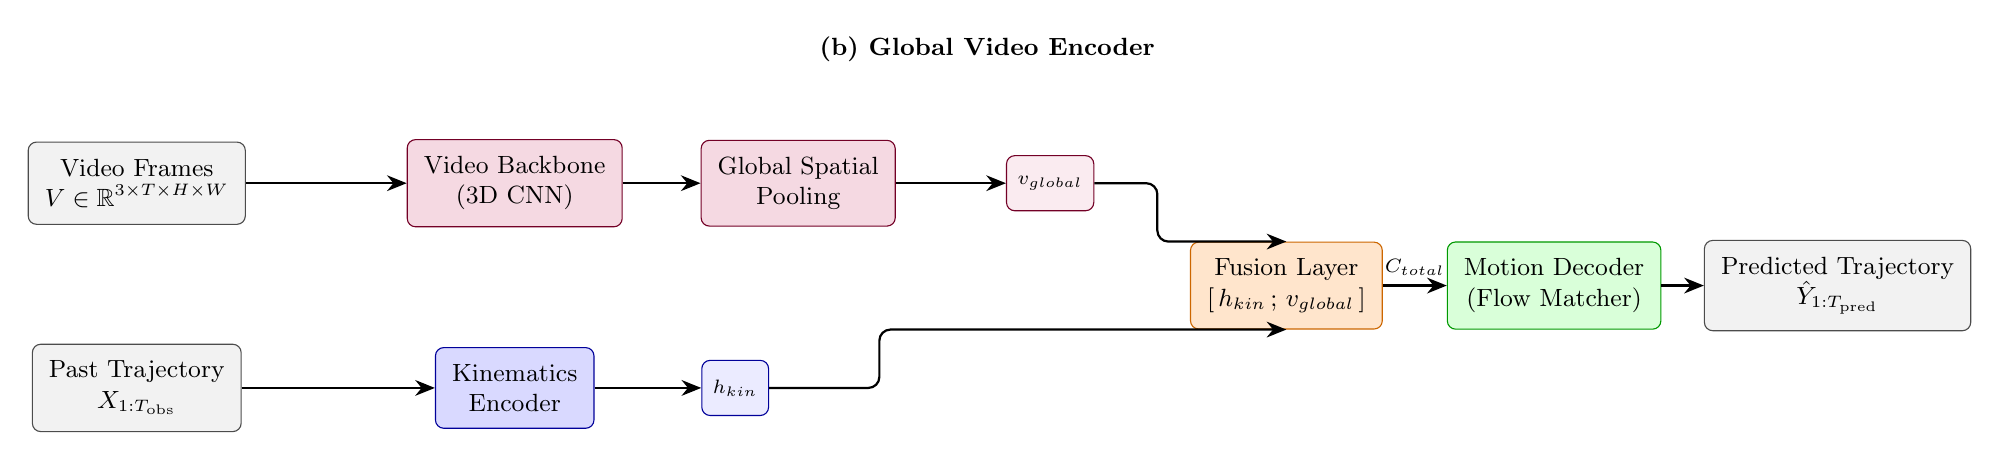
\begin{tikzpicture}
  % ---- kinematics stream (bottom row) ----
  \node[io]  (x)    at (0.0,0.0)   {Past Trajectory\\$X_{1:T_{\mathrm{obs}}}$};
  \node[kin] (kenc) at (4.8,0.0)   {Kinematics\\Encoder};
  \node[vec] (h)    at (7.6,0.0)   {$h_{kin}$};

  % ---- visual stream (top row) ----
  \node[io]   (v)     at (0.0,2.6)  {Video Frames\\$V\in\mathbb{R}^{3\times T\times H\times W}$};
  \node[vid]  (bb)    at (4.8,2.6)  {Video Backbone\\(3D CNN)};
  \node[vid]  (pool)  at (8.4,2.6)  {Global Spatial\\Pooling};
  \node[vecv] (vglob) at (11.6,2.6) {$v_{global}$};

  % ---- fusion + decoder ----
  \node[fuse] (fus) at (14.6,1.3) {Fusion Layer\\$[\,h_{kin}\,;\,v_{global}\,]$};
  \node[dec]  (dec) at (18.0,1.3) {Motion Decoder\\(Flow Matcher)};
  \node[io]   (y)   at (21.6,1.3) {Predicted Trajectory\\$\hat{Y}_{1:T_{\mathrm{pred}}}$};

  % ---- stream arrows ----
  \draw[arrow] (x)    -- (kenc);
  \draw[arrow] (kenc) -- (h);
  \draw[arrow] (v)    -- (bb);
  \draw[arrow] (bb)   -- (pool);
  \draw[arrow] (pool) -- (vglob);

  % ---- merge into fusion ----
  \draw[arrow] (h.east)     -- ++(1.4,0) |- (fus.south);
  \draw[arrow] (vglob.east) -- ++(0.8,0) |- (fus.north);

  \draw[arrow] (fus) -- (dec) node[midway, above, font=\scriptsize] {$C_{total}$};
  \draw[arrow] (dec) -- (y);

  \node[title] at (10.8,4.3) {(b) Global Video Encoder};
\end{tikzpicture}
\end{document}
